\subsection{Kiểm chứng xác thực và phân quyền}
\begin{table}[htbp]\centering\small
\begin{minipage}[t]{.69\linewidth}\vspace{0pt}
\begin{tabularx}{\linewidth}{|p{.13\linewidth}|X|}\hline
\textbf{Ca} & \textbf{Tiêu chí kiểm chứng}\\\hline
AUTH-01 & Đăng ký gửi kèm role BARISTA vẫn tạo CUSTOMER, không tự nâng quyền.\\\hline
AUTH-02 & Login và /auth/me trả vai trò đúng, không có passwordHash.\\\hline
AUTH-03 & Cùng token, đổi role trong database làm quyền gọi /staff/orders thay đổi ở request tiếp theo.\\\hline
AUTH-04 & Route staff thiếu token trả 401; CUSTOMER có token bị 403.\\\hline
AUTH-05 & Khách khác không đọc/hủy/check giao dịch của chủ đơn; dữ liệu và kho không bị thay đổi bởi yêu cầu bị chặn.\\\hline
AUTH-06 & Tiêu chí xác thực token: token sai chữ ký hoặc hết hạn không được đi vào nghiệp vụ được bảo vệ.\\\hline
\end{tabularx}
\end{minipage}\hfill
\begin{minipage}[t]{.27\linewidth}\vspace{0pt}
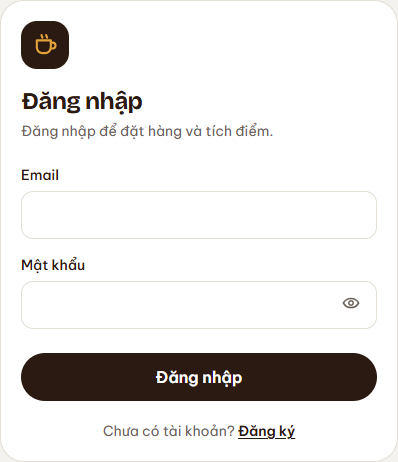
\includegraphics[width=\linewidth]{assets/auth/login-ui.png}
\end{minipage}
\caption{Tiêu chí kiểm chứng quyền và form đăng nhập chụp từ frontend, không có thông tin tài khoản thật}
\end{table}

Ba ca đầu được hiện thực trong \path{test/auth-roles.e2e-spec.ts}. Kiểm tra staff, chủ đơn và giao dịch được phân bố trong các bộ staff-orders, inventory-snapshot và VNPay. AUTH-06 mô tả tiêu chí của cấu hình strategy kiểm chữ ký/hạn; bảng tiêu chí không thay thế log chạy test. Kết quả bộ hồi quy được trình bày theo phạm vi tại mục~\ref{sec:inventory-tests}, không bổ sung số liệu chạy mới ở phần này.

